\section[力学量算符的对易关系式]{力学量算符的对易关系式} \label{sec:03.06} % 
% \makebox[5em][s]{} % 短题目拉间距

许多量子力学问题都涉及到力学蜇算符之间的对易关系式.最基本的就是位置算符和动量算符之间的对易关系式(见$\S$\ref{sec:03.02}):
\eqindent{10}
\begin{empheq}{align}	%1,2,3
	\hat{p_{x}}\hat{p_{y}}-\hat{p_{y}}\hat{p_{x}}=0	\label{eq36.1} \\%1
	\hat{x}\hat{p_{x}}-\hat{p_{x}}\hat{x}=i\hbar	\label{eq36.2} \\%2
	\hat{x}\hat{p_{y}}-\hat{p_{y}}\hat{x}=0			\label{eq36.3}	 %3
\end{empheq}
等等.为了便于运算,定义算符$\hat{A},\hat{B}$之间的对易式(又称量子括号):
\begin{empheq}{equation}\label{eq36.4}
	[\hat{A},\hat{B}]\equiv\hat{A}\hat{B}-\hat{B}\hat{A}
\end{empheq}\eqnormal
\eqindent{12}
则\eqref{eq36.1}、\eqref{eq36.2}、\eqref{eq36.3}式可以写成
\begin{empheq}{align*}	%1',2',3'
	[\hat{p_{x}},\hat{p_{y}}]&=0		\tag{$3.6.1^{\prime}$} \label{eq36.1'} \\
	[\hat{x}\hat{p_{x}}]&=i\hbar		\tag{$3.6.2^{\prime}$} \label{eq36.2'} \\
	[\hat{x}\hat{p_{y}}]&=0			\tag{$3.6.3^{\prime}$} \label{eq36.3'}
\end{empheq}\eqnormal
根据定义\eqref{eq36.4}式,容易证明以下运算规则:
\eqindent{6}
\begin{gather}
	[\hat{A},\hat{B}]=-[\hat{B},\hat{A}]	\label{eq36.5}\\ %5
	[\hat{A},\hat{B}+\hat{C}]=[\hat{A},\hat{B}]+[\hat{A},\hat{C}]	\label{eq36.6}\\ %6
	[\hat{A}+\hat{B},\hat{C}]=[\hat{A},\hat{C}]+[\hat{B},\hat{C}]	\label{eq36.7}\\ %7
	[\hat{A},\hat{B}\hat{C}]=[\hat{A},\hat{B}]\hat{C}+\hat{B}[\hat{A},\hat{C}]	\label{eq36.8}\\ %8
	[\hat{A}\hat{B},\hat{C}]=[\hat{A},\hat{C}]\hat{B}+\hat{A}[\hat{B},\hat{C}]	\label{eq36.9}\\ %9
	[\hat{A},[\hat{B},\hat{C}]]+[\hat{B}[\hat{C},\hat{A}]]+[\hat{C}[\hat{A},\hat{B}]]=0	\label{eq36.10} %10		
\end{gather}
熟练地掌握这些公式,计算就能进行得正确而迅速.例如利用\eqref{eq36.8}式及\eqref{eq36.2'}式,
可得
\begin{align}%11,12
	[\hat{x},\hat{p_{x}}^{2}] &=[\hat{x},\hat{p_{x}}]\hat{p_{x}}+\hat{p_{x}}[\hat{x},\hat{p_{x}}]=2i\hbar\hat{p_{x}}	\label{eq36.11}\\ %11
	[\hat{x},\hat{p_{x}}^{3}] &=[\hat{x},\hat{p_{x}}]\hat{p_{x}}^{2}+\hat{p_{x}}[\hat{x},\hat{p_{x}}^{2}]=3i\hbar\hat{p_{x}}^{2}	\label{eq36.12} %12
\end{align}\eqnormal
依此类推,对于任何正整数$n$,可证
\begin{empheq}{equation}\label{eq36.13}
	[\hat{x},\hat{p_{x}}^{n}]=i\hbar n\hat{p_{x}}^{n-1}=i\hbar\frac{\partial\hat{p_{x}}^{n}}{\partial\hat{p_{x}}}
\end{empheq}
再考虑到\eqref{eq36.3'}式,可知对于任何可以展开成$\hat{p_{x}},\hat{p_{y}},\hat{p_{z}}$正幕级数的算符$\hat{F(\boldsymbol{p})}$,有
下列对易关系式:
\begin{empheq}{equation}\label{eq36.14}
	[\hat{x},\hat{F(\boldsymbol{p})}]=i\hbar\frac{\partial\hat{F}}{\partial\hat{p_{x}}}
\end{empheq}
类似地,对于任意函数(作为算符)$f(\boldsymbol{r})$,有对易式
\begin{empheq}{equation}\label{eq36.15}
	[\hat{p_{x}},f(\boldsymbol{r})]=-i\hbar\frac{\partial f}{\partial x}
\end{empheq}

与轨道角动量算符$\hat{\boldsymbol{L}}=\boldsymbol{r}\times\boldsymbol{p}$有关的对易式应用极广,例如:
\eqindent{6}
\begin{empheq}{align}%16,17,18
	&[\hat{x},\hat{L_{x}}]=[\hat{x},\hat{y}\hat{p_{z}}]-[\hat{x},\hat{z}\hat{p_{y}}]=0	\label{eq36.16}\\
	&[\hat{x},\hat{L_{y}}]=[\hat{x},\hat{z}\hat{p_{x}}]-[\hat{x},\hat{x}\hat{p_{z}}]=\hat{z}[\hat{x},\hat{p_{x}}]=i\hbar\hat{z}	\label{eq36.17}\\
	&[\hat{L_{x}},\hat{y}]=[\hat{y}\hat{p_{z}},\hat{y}]-[\hat{z}\hat{p_{y}},\hat{y}]=-\hat{z}[\hat{p_{y}},\hat{y}]=i\hbar\hat{z}	\label{eq36.18}
\end{empheq}
类似地,可以证明
\begin{empheq}{equation}\label{eq36.19}
	[\hat{p_{x}},\hat{L_{x}}]=0,\quad[\hat{p_{x}},\hat{L_{y}}]=[\hat{L_{x}},\hat{p_{y}}]=i\hbar\hat{p_{z}}
\end{empheq}\eqnormal
等等.以上各式经过$(x\rightarrow y,y\rightarrow z,z\rightarrow x)$轮换后,仍旧成立.例如,\eqref{eq36.17}式和\eqref{eq36.18}式的轮换式是
\begin{empheq}{align*}
	[\hat{y},\hat{L_{z}}]=[\hat{L_{y}},\hat{z}]=i\hbar\hat{x}	\tag{$3.6.17^{\prime}$} \label{eq36.17'} \\
	[\hat{z},\hat{L_{x}}]=[\hat{L_{z}},\hat{x}]=i\hbar\hat{y}	\tag{$3.6.18^{\prime}$} \label{eq36.18'} 
\end{empheq}
\eqref{eq36.16}式的轮换式是
\begin{empheq}{equation*}\label{eq36.16'}
	[\hat{y},\hat{L_{y}}]=0,\quad [\hat{z},\hat{L_{z}}]=0	\tag{$3.6.16^{\prime}$} 
\end{empheq}

利用以上各式,就可以计算角动量算符$\hat{\boldsymbol{L}}$的各个分量之间的对易式,例如:
\eqindent{6}
\begin{empheq}{equation}\label{eq36.20}
	\begin{aligned}
		[\hat{L_{x}},\hat{L_{y}}]&=[\hat{y}\hat{p_{z}},\hat{L_{y}}]-[\hat{z}\hat{p_{y}},\hat{L_{y}}]	\\
		&=\hat{y}[\hat{p_{z}},\hat{L_{y}}]-[\hat{z},\hat{L_{y}}]\hat{p_{y}}	\\
		&=i\hbar(-\hat{y}\hat{p_{x}}+\hat{x}\hat{p_{y}})=i\hbar\hat{L_{z}}
	\end{aligned}
\end{empheq}\eqnormal
\eqref{eq36.20}式及其轮换式常被写成矢量形式:
\eqindent{12}
\begin{empheq}{equation}\label{eq36.21}
	\boxed{\hat{\boldsymbol{L}}\times\hat{\boldsymbol{L}}=i\hbar\hat{\boldsymbol{L}}}
\end{empheq}\eqnormal
利用\eqref{eq36.20}式或\eqref{eq36.21}式,可以进一步证明:
\begin{empheq}{equation}\label{eq36.22}
	[\hat{L_{\alpha}},\hat{\boldsymbol{L}}^{2}]=0,\quad \alpha=x,y,z
\end{empheq}
写成矢量形式,就是\eqindent{12}
\begin{empheq}{equation*}\label{eq36.22'}
	[\hat{\boldsymbol{L}},\hat{\boldsymbol{L}}^{2}]=0	\tag{$3.6.22^{\prime}$}
\end{empheq}\eqnormal
\eqref{eq36.21}、\eqref{eq36.22}式是角动蜇算符最本质的关系式.尤其是\eqref{eq36.21}式,是经典物理中根本不可能有的关系.在经典物理中,所有物理量都是普通数量,当然都是互相对易的,因此对于任何向量$\boldsymbol{A}$,总有$\boldsymbol{A}\times\boldsymbol{A}=0$.而作为量子力学算符的角动量$\hat{\boldsymbol{L}}$,各分量不对易,满足\eqref{eq36.21}式,由此决定了角动量的一系列异乎寻常的性质.$\S$\ref{sec:04.07}将详细讨论这个问题.

利用\eqref{eq36.16}至\eqref{eq36.19}式容易证明:
\begin{empheq}{equation}\label{eq36.23}
	[\hat{L_{\alpha}},\boldsymbol{r}^{2}]=0,\quad[\hat{L_{\alpha}},\hat{\boldsymbol{p}}^{2}]=0,\quad \alpha=x,y,z
\end{empheq}
亦即
\begin{empheq}{equation*}\label{eq36.23'}
	[\hat{\boldsymbol{L}},\boldsymbol{r}^{2}]=0,\quad [\hat{\boldsymbol{L}},\hat{\boldsymbol{p}}^{2}]=0	\tag{$3.6.23^{\prime}$}
\end{empheq}
利用$\hat{\boldsymbol{L}}$的球坐标表示式[\eqref{eq31.15}式],容易看出
\begin{empheq}{equation}\label{eq36.24}
	[\hat{\boldsymbol{L}},\hat{f(r)}]=0
\end{empheq}
$\hat{f(r)}$是任何径向函数(作为算符).总之,角动量算符$\hat{\boldsymbol{L}}$和任何标量(转动不变量)算符对易.

\example 选定任意两个空间方向,以$n,m$表示这两个方向的单位矢量:
\begin{empheq}{equation*}
	\boldsymbol{n}=(n_{x},n_{y},n_{z}),\quad\boldsymbol{m}=(m_{x},m_{y},m_{z})
\end{empheq}
定义角动量算符在$\boldsymbol{n},\boldsymbol{m}$方向的投影
\begin{empheq}{align*}
	\hat{L_{n}}&=\boldsymbol{n}\cdot\hat{\boldsymbol{L}}=n_{x}\hat{L_{x}}+n_{y}\hat{L_{y}}+n_{z}\hat{L_{z}}	\\
	\hat{L_{m}}&=\boldsymbol{m}\cdot\hat{\boldsymbol{L}}=m_{x}\hat{L_{x}}+m_{y}\hat{L_{y}}+m_{z}\hat{L_{z}}
\end{empheq}
试计算对易式$[\hat{L_{n}},\hat{L_{m}}]$.

\begin{wrapfigure}[6]{r}{7em}
	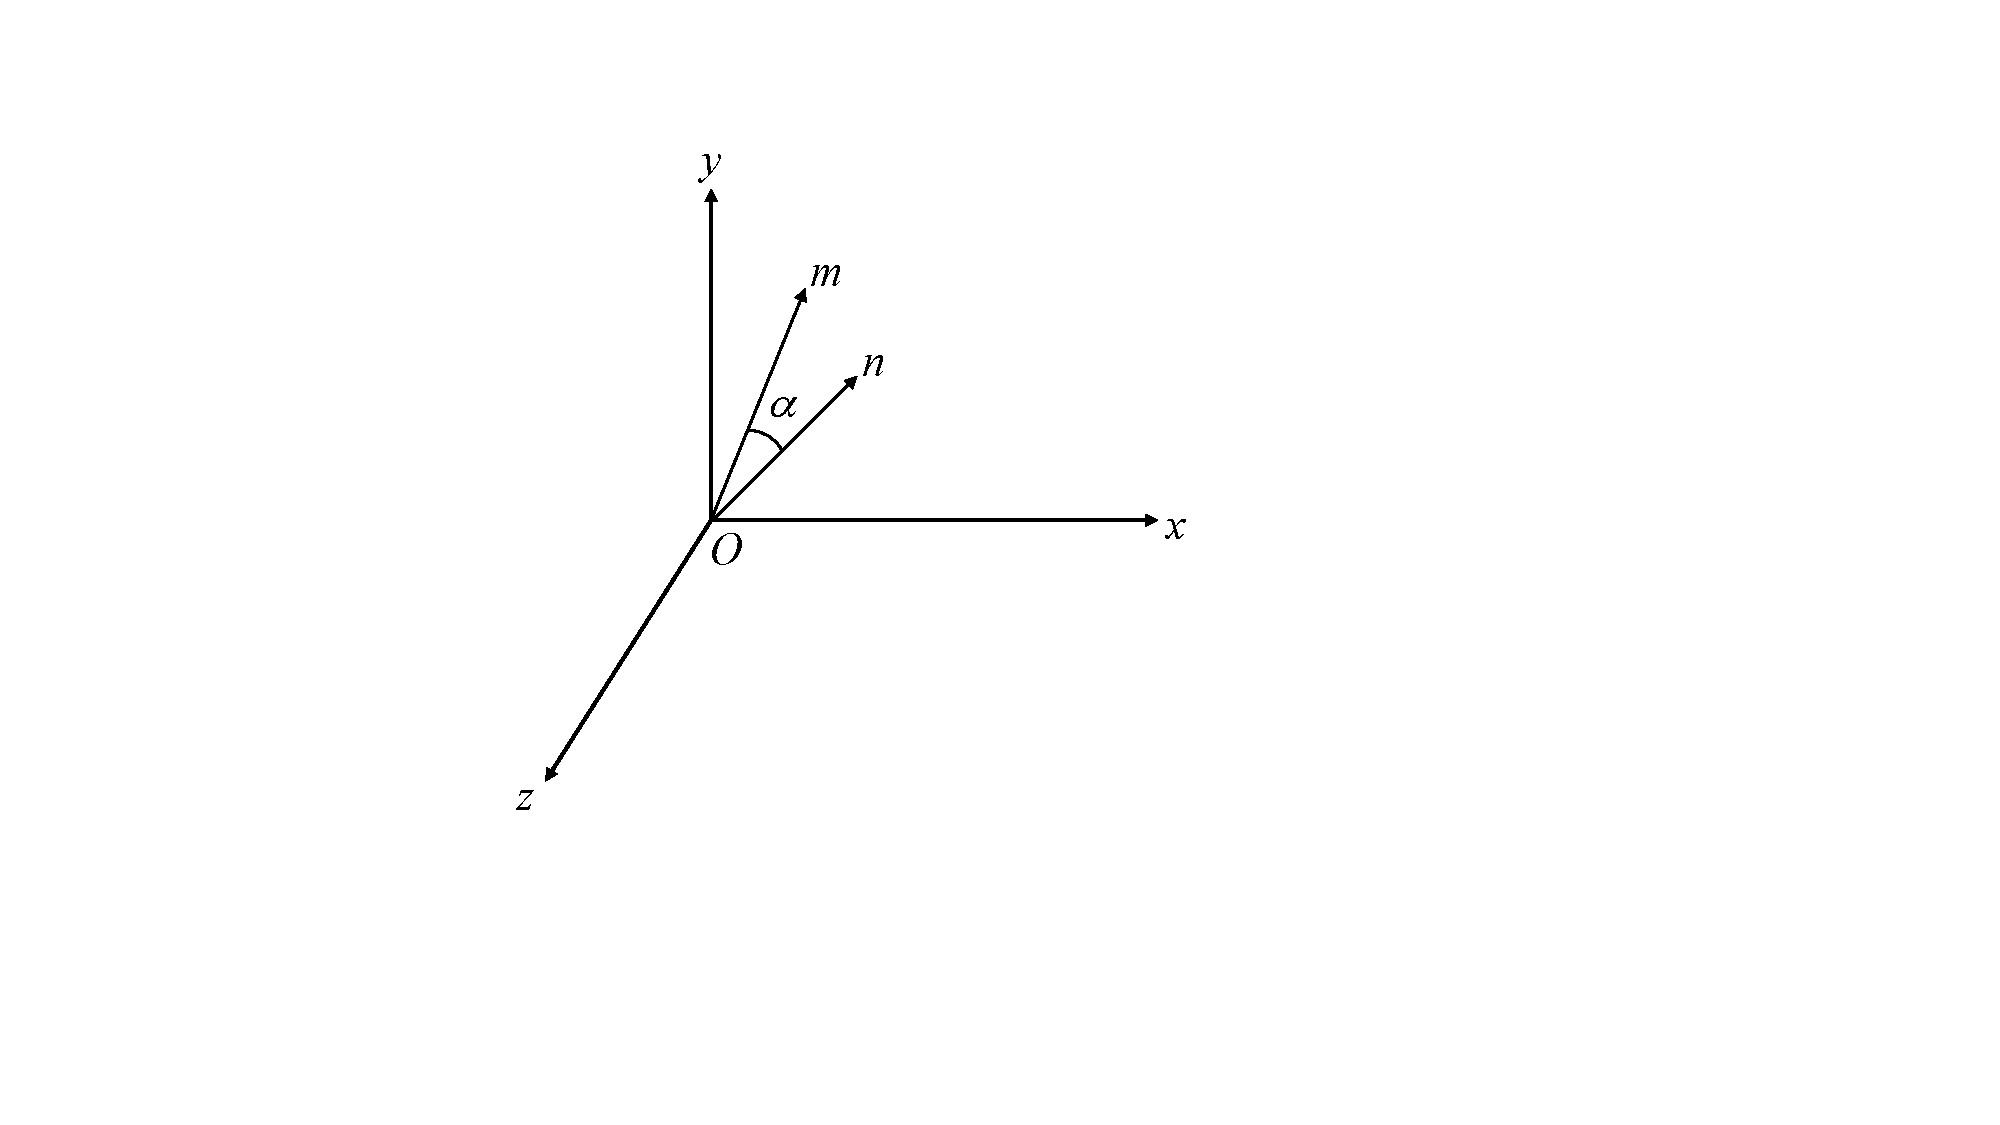
\includegraphics[width=3cm]{QM file/figure/3-3}
	\caption{}\label{fig.3-3}
\end{wrapfigure}

\solution 利用基本对易式\eqref{eq36.21},可得
\eqindent{2}
\begin{align}\label{eq36.25}
	[\hat{L_{n}},\hat{L_{m}}]& = n_{x}m_{y}[\hat{L_{x}},\hat{L_{y}}]+n_{y}m_{x}[\hat{L_{y}},\hat{L_{x}}]+\cdots	\nonumber\\
	&= (n_{x}m_{y}-n_{y}m_{x})i\hbar\hat{L_{z}}+\cdots	\nonumber\\
	&= i\hbar(\boldsymbol{n}\times\boldsymbol{m})_{z}\hat{L_{z}}+\cdots	\nonumber\\
	&= i\hbar(\boldsymbol{n}\times\boldsymbol{m})\cdot\hat{\boldsymbol{L}}
\end{align}\eqnormal
如以$\alpha$表示$(\boldsymbol{n},\boldsymbol{m})$夹角,$\boldsymbol{l}$表示$(\boldsymbol{n}\times\boldsymbol{m})$方向单位矢量,上式可以写成
\begin{empheq}{equation*}\label{eq36.25'}
	[\hat{L_{n}},\hat{L_{m}}]=i\hbar\hat{L_{l}}\sin\alpha
\end{empheq}
如果$\boldsymbol{n},\boldsymbol{m}$在$x-y$平面上,则$\boldsymbol{n}\times\boldsymbol{m}$指向$z$轴,如图\ref{fig.3-3}所示,上式成为
\begin{empheq}{equation}\label{eq36.26}
	[\hat{L_{n}},\hat{L_{m}}]=i\hbar\hat{L_{z}}\sin\alpha
\end{empheq}
其中角$\alpha$定义为由$\boldsymbol{n}$方向开始,沿逆时针方向转到$\boldsymbol{m}$方向所经历的角度($\alpha$可以大于$\pi$).



